%%%%%%%%%%%%%%%%%%%%%%%%%%%%%%%%%%%%%%%%%
% Lachaise Assignment
% LaTeX Template
% Version 1.0 (26/6/2018)
%
% This template originates from:
% http://www.LaTeXTemplates.com
%
% Authors:
% Marion Lachaise & François Févotte
% Vel (vel@LaTeXTemplates.com)
%
% License:
% CC BY-NC-SA 3.0 (http://creativecommons.org/licenses/by-nc-sa/3.0/)
% 
%%%%%%%%%%%%%%%%%%%%%%%%%%%%%%%%%%%%%%%%%

%----------------------------------------------------------------------------------------
%	PACKAGES AND OTHER DOCUMENT CONFIGURATIONS
%----------------------------------------------------------------------------------------

\documentclass{article}

%%%%%%%%%%%%%%%%%%%%%%%%%%%%%%%%%%%%%%%%%
% Lachaise Assignment
% Structure Specification File
% Version 1.0 (26/6/2018)
%
% This template originates from:
% http://www.LaTeXTemplates.com
%
% Authors:
% Marion Lachaise & François Févotte
% Vel (vel@LaTeXTemplates.com)
%
% License:
% CC BY-NC-SA 3.0 (http://creativecommons.org/licenses/by-nc-sa/3.0/)
% 
%%%%%%%%%%%%%%%%%%%%%%%%%%%%%%%%%%%%%%%%%

%----------------------------------------------------------------------------------------
%	PACKAGES AND OTHER DOCUMENT CONFIGURATIONS
%----------------------------------------------------------------------------------------

\usepackage{amsmath,amsfonts,stmaryrd,amssymb} % Math packages

\usepackage{enumerate} % Custom item numbers for enumerations

\usepackage[ruled]{algorithm2e} % Algorithms

\usepackage[framemethod=tikz]{mdframed} % Allows defining custom boxed/framed environments

\usepackage{listings} % File listings, with syntax highlighting
\lstset{
	basicstyle=\ttfamily, % Typeset listings in monospace font
}

\usepackage{pdfpages}


%----------------------------------------------------------------------------------------
%	DOCUMENT MARGINS
%----------------------------------------------------------------------------------------

\usepackage{geometry} % Required for adjusting page dimensions and margins

\geometry{
	paper=a4paper, % Paper size, change to letterpaper for US letter size
	top=2.5cm, % Top margin
	bottom=3cm, % Bottom margin
	left=2.5cm, % Left margin
	right=2.5cm, % Right margin
	headheight=14pt, % Header height
	footskip=1.5cm, % Space from the bottom margin to the baseline of the footer
	headsep=1.2cm, % Space from the top margin to the baseline of the header
	%showframe, % Uncomment to show how the type block is set on the page
}

%----------------------------------------------------------------------------------------
%	FONTS
%----------------------------------------------------------------------------------------

\usepackage[utf8]{inputenc} % Required for inputting international characters
\usepackage[T1]{fontenc} % Output font encoding for international characters

\usepackage{XCharter} % Use the XCharter fonts

%----------------------------------------------------------------------------------------
%	COMMAND LINE ENVIRONMENT
%----------------------------------------------------------------------------------------

% Usage:
% \begin{commandline}
%	\begin{verbatim}
%		$ ls
%		
%		Applications	Desktop	...
%	\end{verbatim}
% \end{commandline}

\mdfdefinestyle{commandline}{
	leftmargin=10pt,
	rightmargin=10pt,
	innerleftmargin=15pt,
	middlelinecolor=black!50!white,
	middlelinewidth=2pt,
	frametitlerule=false,
	backgroundcolor=black!5!white,
	frametitle={Command Line},
	frametitlefont={\normalfont\sffamily\color{white}\hspace{-1em}},
	frametitlebackgroundcolor=black!50!white,
	nobreak,
}

% Define a custom environment for command-line snapshots
\newenvironment{commandline}{
	\medskip
	\begin{mdframed}[style=commandline]
}{
	\end{mdframed}
	\medskip
}

%----------------------------------------------------------------------------------------
%	FILE CONTENTS ENVIRONMENT
%----------------------------------------------------------------------------------------

% Usage:
% \begin{file}[optional filename, defaults to "File"]
%	File contents, for example, with a listings environment
% \end{file}

\mdfdefinestyle{file}{
	innertopmargin=1.6\baselineskip,
	innerbottommargin=0.8\baselineskip,
	topline=false, bottomline=false,
	leftline=false, rightline=false,
	leftmargin=2cm,
	rightmargin=2cm,
	singleextra={%
		\draw[fill=black!10!white](P)++(0,-1.2em)rectangle(P-|O);
		\node[anchor=north west]
		at(P-|O){\ttfamily\mdfilename};
		%
		\def\l{3em}
		\draw(O-|P)++(-\l,0)--++(\l,\l)--(P)--(P-|O)--(O)--cycle;
		\draw(O-|P)++(-\l,0)--++(0,\l)--++(\l,0);
	},
	nobreak,
}

% Define a custom environment for file contents
\newenvironment{file}[1][File]{ % Set the default filename to "File"
	\medskip
	\newcommand{\mdfilename}{#1}
	\begin{mdframed}[style=file]
}{
	\end{mdframed}
	\medskip
}

%----------------------------------------------------------------------------------------
%	NUMBERED QUESTIONS ENVIRONMENT
%----------------------------------------------------------------------------------------

% Usage:
% \begin{question}[optional title]
%	Question contents
% \end{question}

\mdfdefinestyle{question}{
	innertopmargin=1.2\baselineskip,
	innerbottommargin=0.8\baselineskip,
	roundcorner=5pt,
	nobreak,
	singleextra={%
		\draw(P-|O)node[xshift=1em,anchor=west,fill=white,draw,rounded corners=5pt]{%
		Question \theQuestion\questionTitle};
	},
}

\newcounter{Question} % Stores the current question number that gets iterated with each new question

% Define a custom environment for numbered questions
\newenvironment{question}[1][\unskip]{
	\bigskip
	\stepcounter{Question}
	\newcommand{\questionTitle}{~#1}
	\begin{mdframed}[style=question]
}{
	\end{mdframed}
	\medskip
}

%----------------------------------------------------------------------------------------
%	WARNING TEXT ENVIRONMENT
%----------------------------------------------------------------------------------------

% Usage:
% \begin{warn}[optional title, defaults to "Warning:"]
%	Contents
% \end{warn}

\mdfdefinestyle{warning}{
	topline=false, bottomline=false,
	leftline=false, rightline=false,
	nobreak,
	singleextra={%
		\draw(P-|O)++(-0.5em,0)node(tmp1){};
		\draw(P-|O)++(0.5em,0)node(tmp2){};
		\fill[black,rotate around={45:(P-|O)}](tmp1)rectangle(tmp2);
		\node at(P-|O){\color{white}\scriptsize\bf !};
		\draw[very thick](P-|O)++(0,-1em)--(O);%--(O-|P);
	}
}

% Define a custom environment for warning text
\newenvironment{warn}[1][Warning:]{ % Set the default warning to "Warning:"
	\medskip
	\begin{mdframed}[style=warning]
		\noindent{\textbf{#1}}
}{
	\end{mdframed}
}

%----------------------------------------------------------------------------------------
%	INFORMATION ENVIRONMENT
%----------------------------------------------------------------------------------------

% Usage:
% \begin{info}[optional title, defaults to "Info:"]
% 	contents
% 	\end{info}

\mdfdefinestyle{info}{%
	topline=false, bottomline=false,
	leftline=false, rightline=false,
	nobreak,
	singleextra={%
		\fill[black](P-|O)circle[radius=0.4em];
		\node at(P-|O){\color{white}\scriptsize\bf i};
		\draw[very thick](P-|O)++(0,-0.8em)--(O);%--(O-|P);
	}
}

% Define a custom environment for information
\newenvironment{info}[1][Info:]{ % Set the default title to "Info:"
	\medskip
	\begin{mdframed}[style=info]
		\noindent{\textbf{#1}}
}{
	\end{mdframed}
}
 % Include the file specifying the document structure and custom commands

%----------------------------------------------------------------------------------------
%	ASSIGNMENT INFORMATION
%----------------------------------------------------------------------------------------

\title{Project: Solving proximity constraints} % Title of the assignment

\author{Jan-Michael Holzinger\thanks{jan.holzinger@gmx.at} \and Sophie Hofmanninger\thanks{sophie@hofmanninger.co.at}} % Author name and email address

\date{JKU Linz --- SS2019} % University, school and/or department name(s) and a date

%----------------------------------------------------------------------------------------

\begin{document}

\maketitle % Print the title

%----------------------------------------------------------------------------------------
%	INTRODUCTION
%----------------------------------------------------------------------------------------

\begin{center}
\begin{tabular}[h]{|l|l|l|}
\hline
Version Number & Changes Summary & Author\\
\hline
0.1 & & Jan-Michael\\
\hline
0.2 & added System Model & Jan-Michael\\
\hline
0.3 & modified Parser, added Workflow & Jan-Michael\\
\hline
0.4 & add ConstraintSimplification & Sophie\\
\hline
0.5 & Proximity Relation (as Matrix) added & Jan-Michael\\
\hline
0.6 & update system model, update matrix & Sophie\\
\hline
0.7 & added UML & Jan-Michael\\
\hline
0.8 & added User Interfaces & Jan-Michael\\
\hline
0.9 & minor changes in matrix description & Sophie\\
& update constraint simplification&\\
\hline
0.10 & updated UML files & Jan-Michael\\
\hline
0.11 & added Input Checker & Jan-Michael\\
\hline
\end{tabular}

\end{center}
\section{System Overview}

We split the problem in 4 (5) smaller tasks:
\begin{enumerate}
	\item Input Processing,
	\item Pre-Unification,
	\item Constraint Simplification,
	\item Output.
	\item [O.] Web-Integration.
\end{enumerate}

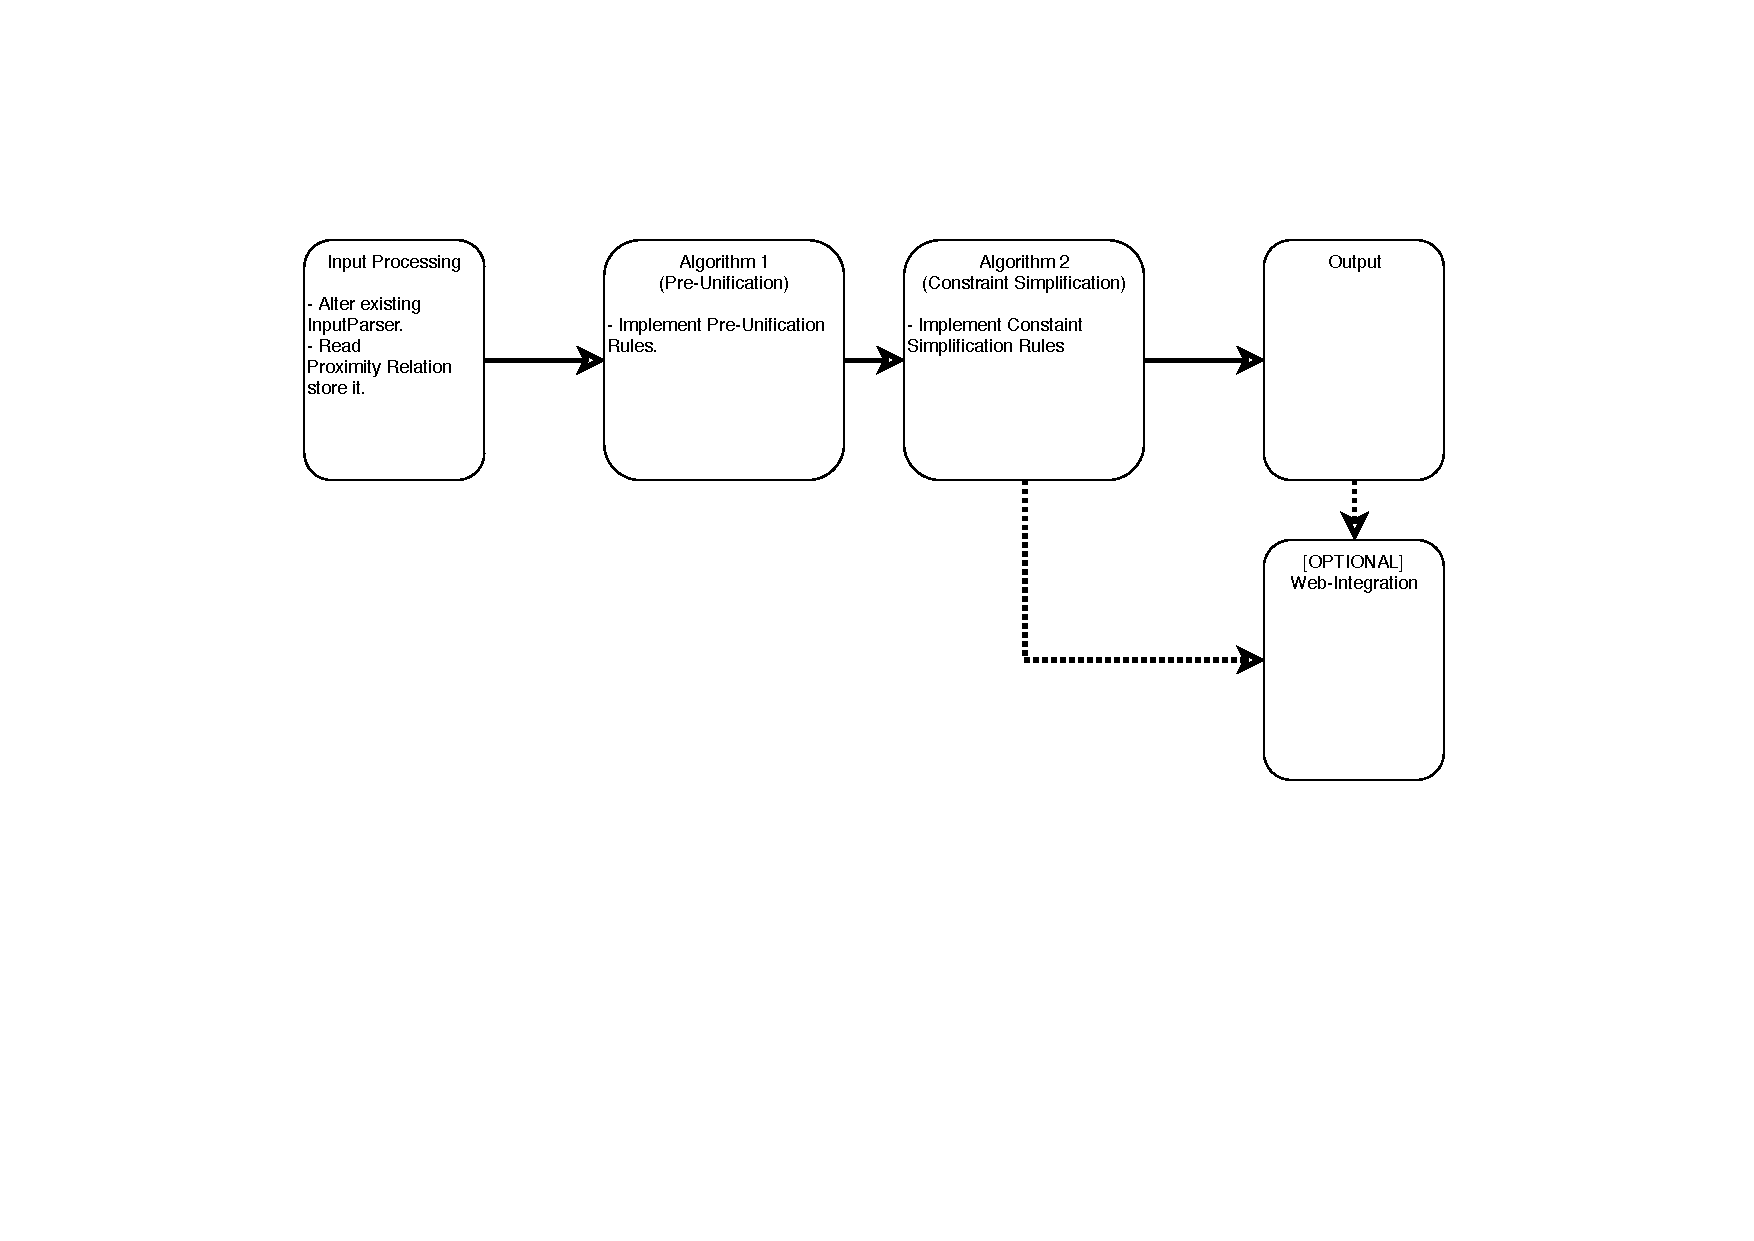
\includepdf[pages=-]{Model}




%----------------------------------------------------------------------------------------
%	PROBLEM 1
%----------------------------------------------------------------------------------------

\subsection{Input Processing} 
\subsubsection{InputParser}
The first idea here is to copy, alter and extend the existing code, in the class InputParser.
\\ \ \\
\noindent
\subsubsection{Input Checker}
We want to be able to check the input for example for missing parenthesis and so on. Therefore we will allow the user to specify an InputChecker. The idea is, to create an Interface, with just a method check(String):boolean. This then can be implemented by the implementation of the checkers.
\subsubsection{Proximity Relations}
For the Proximity Relations \(\mathcal{R}\) and the \(\lambda\)\textit{-cut} we have the following idea:\\
\begin{enumerate}
	\item We try to get the number of function symbols with the same arity. 
	\item We let the user input the values to construct a symmetric matrix that consists of values in \([0,1]\). This matrix must have a 1 in the main diagonal. All values below are 0. Therefore they will not be stored in the implementation.
	\item We let the user (later) input \(\lambda\in[0,1]\) and calculate the set \(\mathcal{R}_\lambda\).
\end{enumerate}

\noindent
The current implementation of InputParser creates a list of all Functions. This list is then sorted by arity, i.e. let \(f,g\) be functions with arity \(a,b \in \mathbb{N}\) respectively. Then \(a<b \Rightarrow f\prec g\).\\
Let now \(n\in\mathbb{N}\) be the size of the list, the list then represents the caption of a \(n\times n\) matrix. Assume the problem contains functions with arity 0,1,\dots,m. Let \(k_l\) be the number of Functions with arity \(l\). Then 
\[\sum_{l=0}^{m}k_l=n.\]
The matrix then looks like 
\[\kbordermatrix{
    & f_{0_1} & f_{0_2} & \dots & f_{0_{k_0}} & f_{1_1} & f_{1_2} & \dots & f_{1_{k_1}} & \dots & f_{m_1} & f_{m_2} & \dots & f_{m_{k_m}}\\
    f_{0_1}     & 1 & (*) & (*) & (*) & 0 & 0 & 0 & 0 & 0 & 0 & 0 & 0 & 0\\
    f_{0_2}     & * & 1 & (*) & (*) & 0 & 0 & 0 & 0 & 0 & 0 & 0 & 0 & 0\\
    \vdots      & * & * & \ddots & (*) & 0 & 0 & 0 & 0 & 0 & 0 & 0 & 0 & 0\\
    f_{0_{k_0}} & * & * & * & 1 & 0 & 0 & 0 & 0 & 0 & 0 & 0 & 0 & 0\\
    f_{1_1}     & 0 & 0 & 0 & 0 & 1 & (*) & (*) & (*) & 0 & 0 & 0 & 0 & 0\\		
		f_{1_2}     & 0 & 0 & 0 & 0 & * & 1 & (*) & (*) & 0 & 0 & 0 & 0 & 0\\
		\vdots      & 0 & 0 & 0 & 0 & * & * & \ddots & (*) & 0 & 0 & 0 & 0 & 0\\
		f_{1_{k_1}} & 0 & 0 & 0 & 0 & * & * & * & 1 & 0 & 0 & 0 & 0 & 0\\
		\vdots      & 0 & 0 & 0 & 0 & 0 & 0 & 0 & 0 & \ddots & 0 & 0 & 0 & 0\\
		f_{m_1}     & 0 & 0 & 0 & 0 & 0 & 0 & 0 & 0 & 0 & 1 & (*) & (*) & (*)\\
		f_{m_2}     & 0 & 0 & 0 & 0 & 0 & 0 & 0 & 0 & 0 & * & 1 & (*) & (*)\\
		\vdots      & 0 & 0 & 0 & 0 & 0 & 0 & 0 & 0 & 0 & * & * & \ddots & (*)\\
		f_{m_{k_m}} & 0 & 0 & 0 & 0 & 0 & 0 & 0 & 0 & 0 & * & * & * & 1\\
  }\quad,\]
where:
\begin{itemize}
	\item the 1's in the diagonal are fixed, as a function must have proximity 1 to itself,
	\item the 0's are fixed, as functions with different aritys can't be close,
	\item the values where the entry is * must be of the same value as their (*) counterpart, as the matrix is symmetric.
\end{itemize} 
Hence, we only need to get the values for the positions marked with (*). We call such a position ``open case'', and we make a list of open cases. Before asking the user to enter relation values, we will generate the list of open cases inside of the matrix. After generation of the list, we will wait for user input. With the valid user input we will build the proximity relation matrix. \\ \ \\
\noindent
If we want to retrieve a value, i.e. if we want to know \(\mathcal{R}(s_1,s_2)\) for given \(s_1,s_2\), we can call \(getRelation(s_1,s_2)\). To get all relation pairs of \(s_1\), that have a relation value greater or equal to \(\lambda\), the method \(getRelations(s_1,\lambda)\) can be used. Moreover it is possible to get all reation elements of the matirix by calling \(getListOf Functions()\). This will return all \( f_{i_{k_j}}\), where \( 0\leq i \leq m\) and \( 0\leq j \leq m\).
%\[i:= \mathrm{sortedListOfFunctions}.\mathrm{getIndex}(s_1)\quad\text{and}\quad j:= \mathrm{sortedListOfFunctions}.\mathrm{getIndex}(s_2),\]
%and then just get the value at position \((i,j)\).

%------------------------------------------------
\subsection{Algorithms}

We implement the Algorithms in an own class, that has two public  static functions, preUnification and constraintSimplification. The other methods are only used for the construction of the two simplification algorithms and therefore they are private and static. The methods should take two inputs, mandatory an unification problem, and optional a StringBuffer, to log certain events.

\subsubsection{Pre-Unification Algorithm}
The preUnification method consists of a loop, that runs until either \(\mathrm{P}=\emptyset\) or it is detected, that there is no solution to the problem.\\
Inside the loop body, the 7 pre-unification rules are iteratively applied to the first element (which gets popped by doing so). The method returns true, iff the pre-unification was successful.
\\ \ \\
\noindent 
The method changes the problems constraints and pre-unifier accordingly.
	
%------------------------------------------------

\subsubsection{Constraint Simplification Algorithm}
The constraintSimplification method will be called, if the preUnification method returns true. As the preUnification method, the constraintSimplification method consists of a loop. This loop runs until the set of constraints is empty. As input the method needs the problem, more precisely the set of constraints, and the relation matrix \(\mathcal{R}\). If the set of constraints could be simplified, the method returns true and otherwise false.\\
Inside the loop, the seven rules to simplify the constraint set, will be applied. Three of the seven rules are hidden, because the NN2 rule is integrated in the NN1 rule, the Fail1 is implemented in FFS and the Fail2 is integrated in the NN1 rule. Moreover it is possible to run the constraint simplification algorithm with and without logging. 

%----------------------------------------------------------------------------------------
%	PROBLEM 2
%----------------------------------------------------------------------------------------

\subsection{Output}

\section{System Model}
The program consists of 4 packages,
\begin{itemize}
	\item tool
	\item elements
	\item unificationProblem
	\item userInterfaces
\end{itemize}
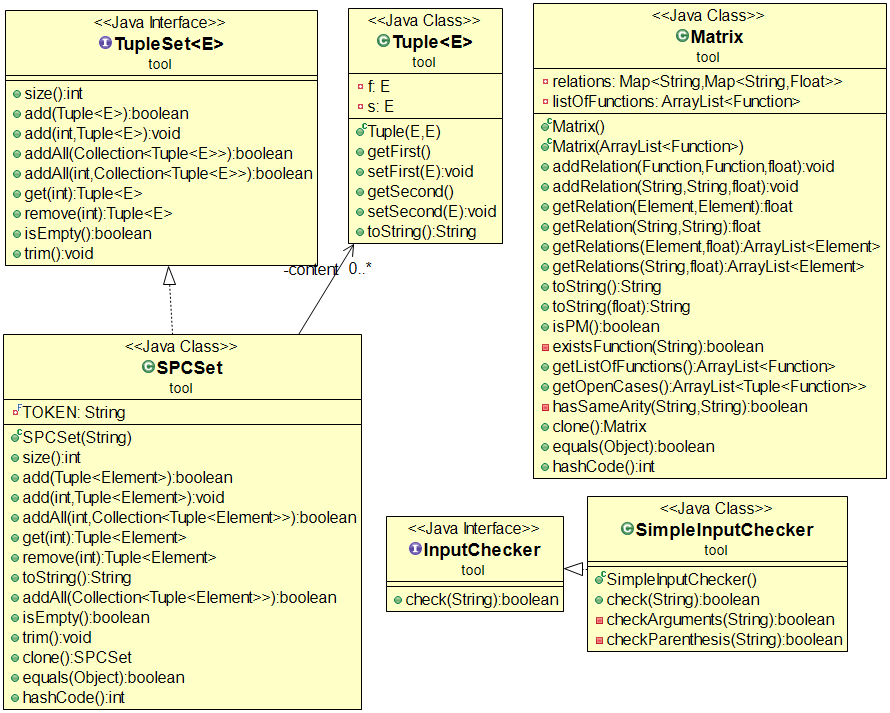
\includegraphics[scale=0.5]{ToolsModel}
\newpage
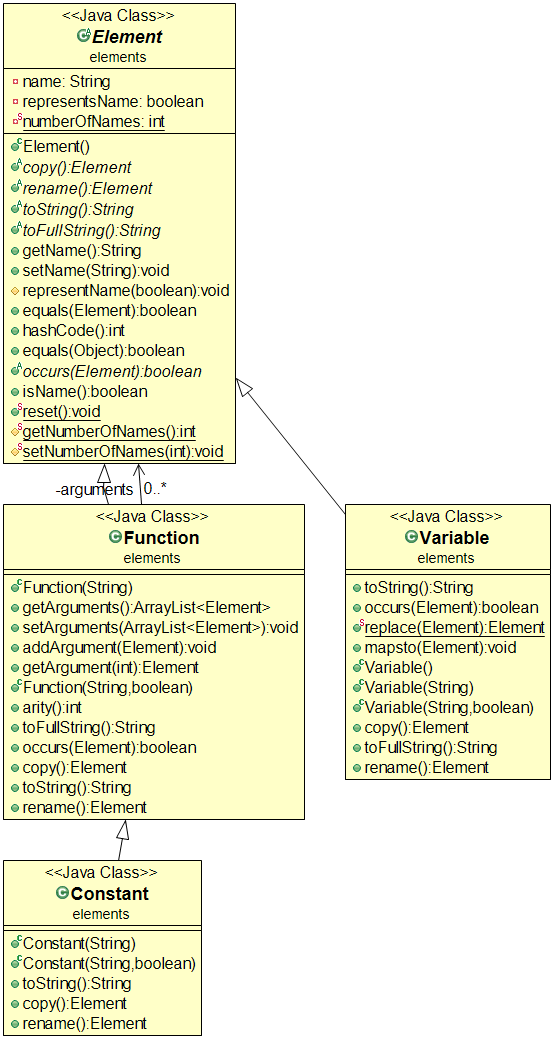
\includegraphics[scale=0.5]{ElementsModel}
\newpage
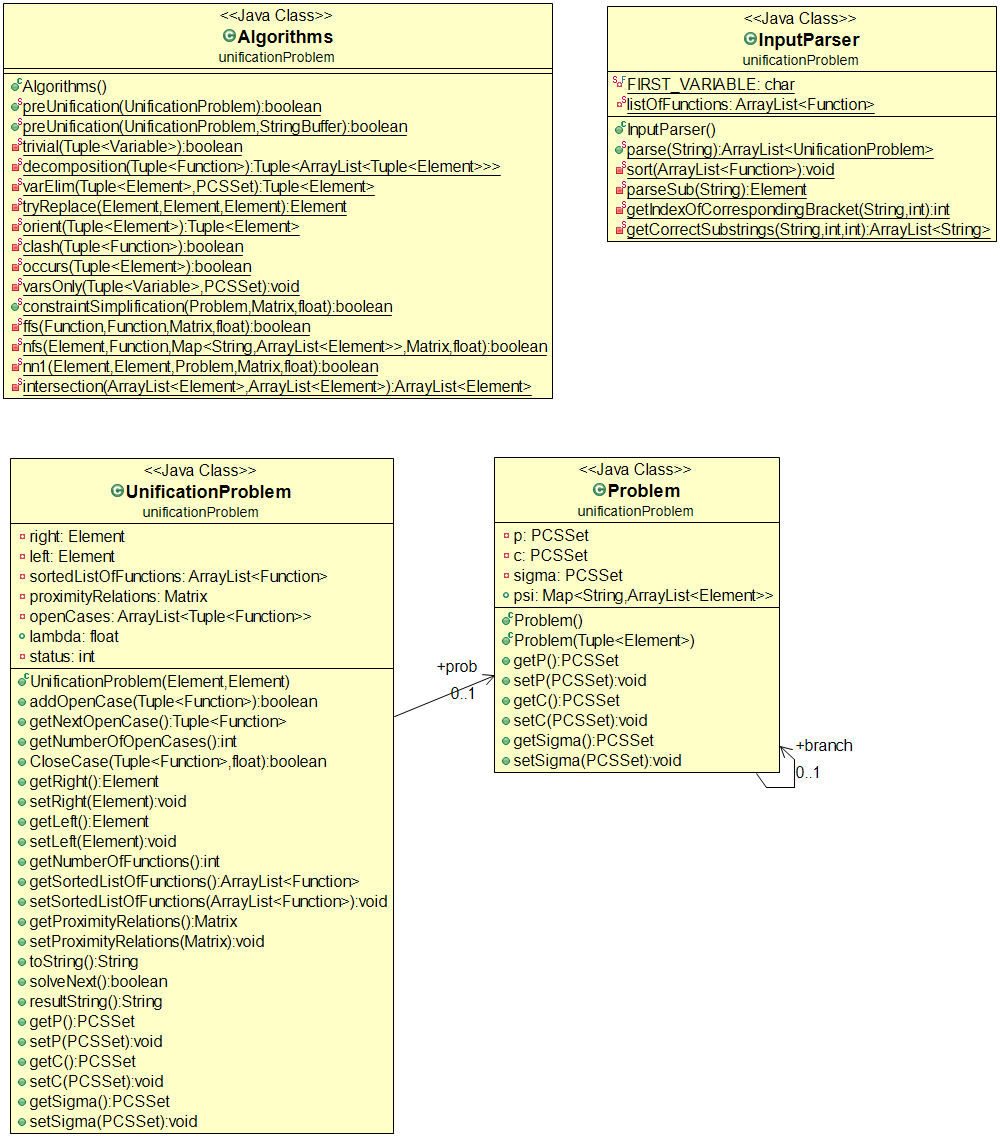
\includegraphics[scale=0.5]{UnificationProblemModel}
\newpage
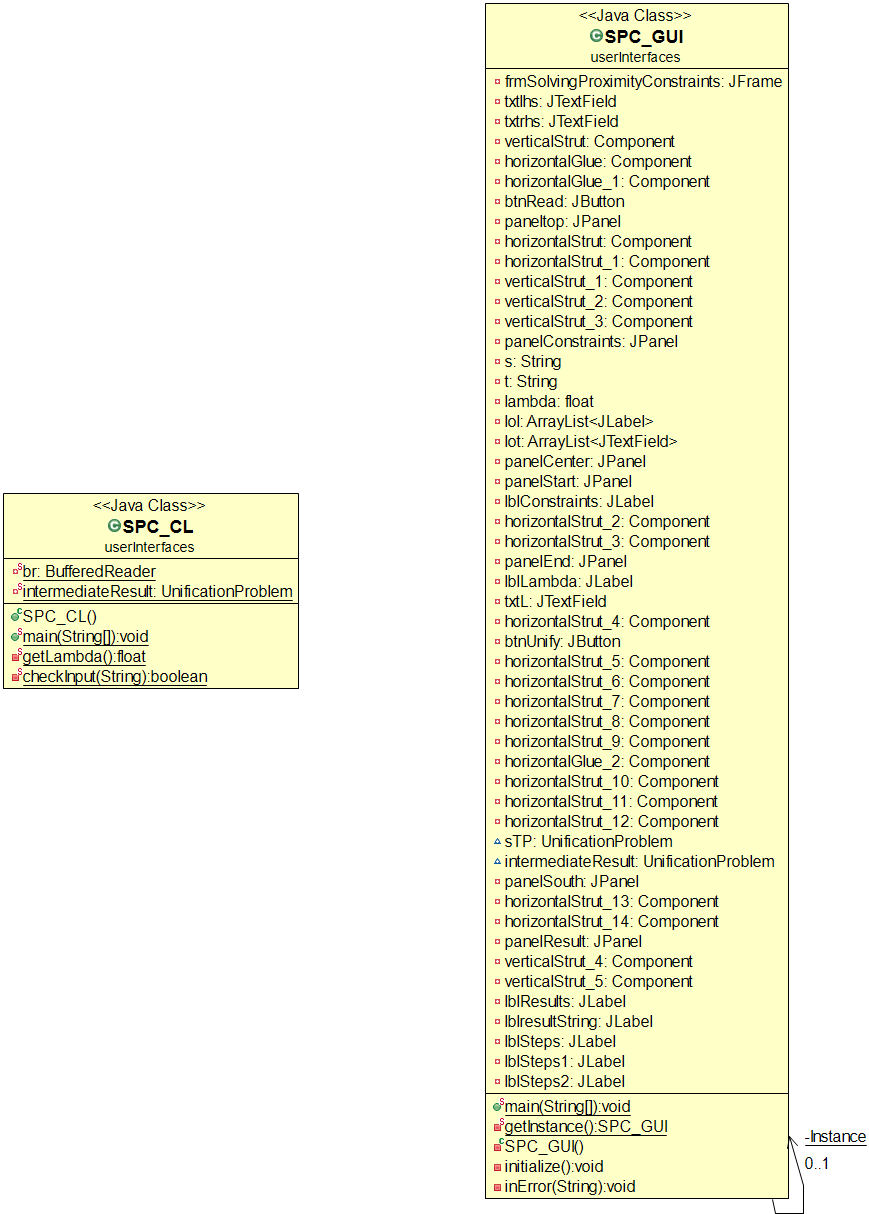
\includegraphics[scale=0.5]{UIModel}


\section{Work Flow}
The typical workflow looks like this:
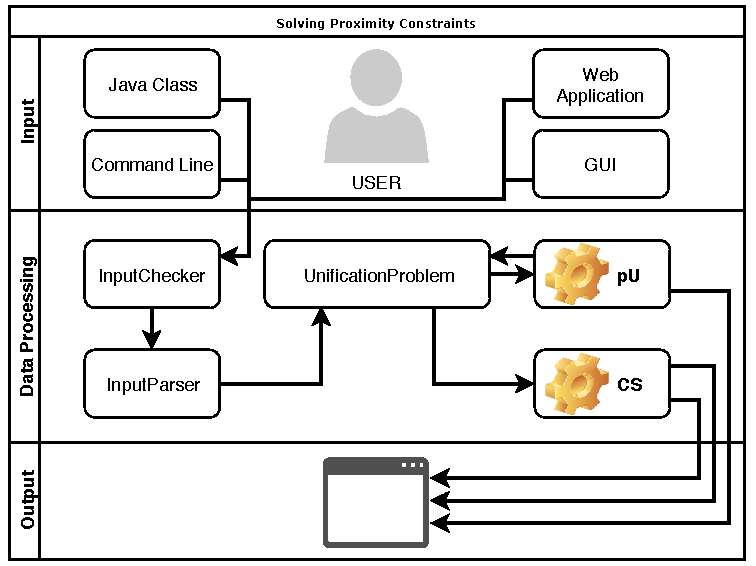
\includepdf[landscape=true, pages=-]{WorkFlow}
% File contents
%\begin{file}[hello.py]
%\begin{lstlisting}[language=Python]
%#! /usr/bin/python
%
%import sys
%sys.stdout.write("Hello World!\n")
%\end{lstlisting}
%\end{file}




% Command-line "screenshot"
%\begin{commandline}
	%\begin{verbatim}
		%$ chmod +x hello.py
		%$ ./hello.py
%
		%Hello World!
	%\end{verbatim}
%\end{commandline}

% Numbered question, with an optional title

%\begin{question}[\itshape (with optional title)]
	%In congue risus leo, in gravida enim viverra id.
%\end{question}

%\begin{question}
	%Quisque ullamcorper placerat ipsum. Cras nibh. Morbi vel justo vitae lacus tincidunt ultrices. Lorem ipsum dolor sit amet, consectetuer adipiscing elit.
%
	%% Subquestions numbered with letters
	%\begin{enumerate}[(a)]
		%\item Do this.
		%\item Do that.
		%\item Do something else.
	%\end{enumerate}
%\end{question}



% Warning text, with a custom title
%\begin{warn}[Notice:]
  %In congue risus leo, in gravida enim viverra id.
%\end{warn}
%\begin{info} % Information block
	%This is an interesting piece of information, to which the reader should pay special attention. 
%\end{info}

% Math equation/formula
%\begin{equation}
%	I = \int_{a}^{b} f(x) \; \text{d}x.
%\end{equation}

%----------------------------------------------------------------------------------------

\end{document}
